\documentclass{ltjsarticle}
\usepackage[scaled]{berasans}
\usepackage[T1]{fontenc}
\usepackage{tikz}
\usetikzlibrary{backgrounds}
\usetikzlibrary{external}
\usetikzlibrary{fit}
\usetikzlibrary{positioning}

\pgfrealjobname{flux}

\definecolor{yellow}{HTML}{FFE53B}
\definecolor{lightblue}{HTML}{76B6C8}
\definecolor{darkgray}{HTML}{434242}
\definecolor{darkgreen}{HTML}{354450}
\definecolor{lightgreen}{HTML}{5FAF6A}

\definecolor{gray}{HTML}{4F4E50}

\tikzset{
  part/.style={
    draw,
    white,
    rectangle,
    rounded corners=5mm,
    minimum width=55mm,
    minimum height=35mm,
    node distance=25mm,
    node font=\sffamily\Huge,
    line width=2mm,
  },
  flow/.style={
    draw,
    >=latex,
    ->,
    yellow,
    line width=1mm,
  },
  action/.style={
    part,
    fill=lightblue,
  },
  dispatcher/.style={
    part,
    fill=darkgray,
  },
  store/.style={
    part,
    fill=darkgreen,
  },
  view/.style={
    part,
    fill=lightgreen,
  },
  background/.style={
    inner xsep=30mm,
    inner ysep=20mm,
    fill=gray,
  },
  explained/.style={
    white,
    node font=\sffamily\huge,
    align=left,
    inner sep=0,
  }
}

\def\basediagram{
  \node (action)     [action]                          {Action};
  \node (dispatcher) [dispatcher,base right=of action] {Dispatcher};
  \node (store)      [store,base right=of dispatcher]  {Store};
  \node (view)       [view,base right=of store]        {View};

  \path [flow] (action) -- (dispatcher);
  \path [flow] (dispatcher) -- (store);
  \path [flow] (store) -- (view);
}

\def\diagram{
  \basediagram

  \node (action2) [action, above=10mm of store] {Action};
  \path [flow] (view) |- (action2) -| (dispatcher);
}

\begin{document}

\beginpgfgraphicnamed{flux-simple-f8-diagram}%
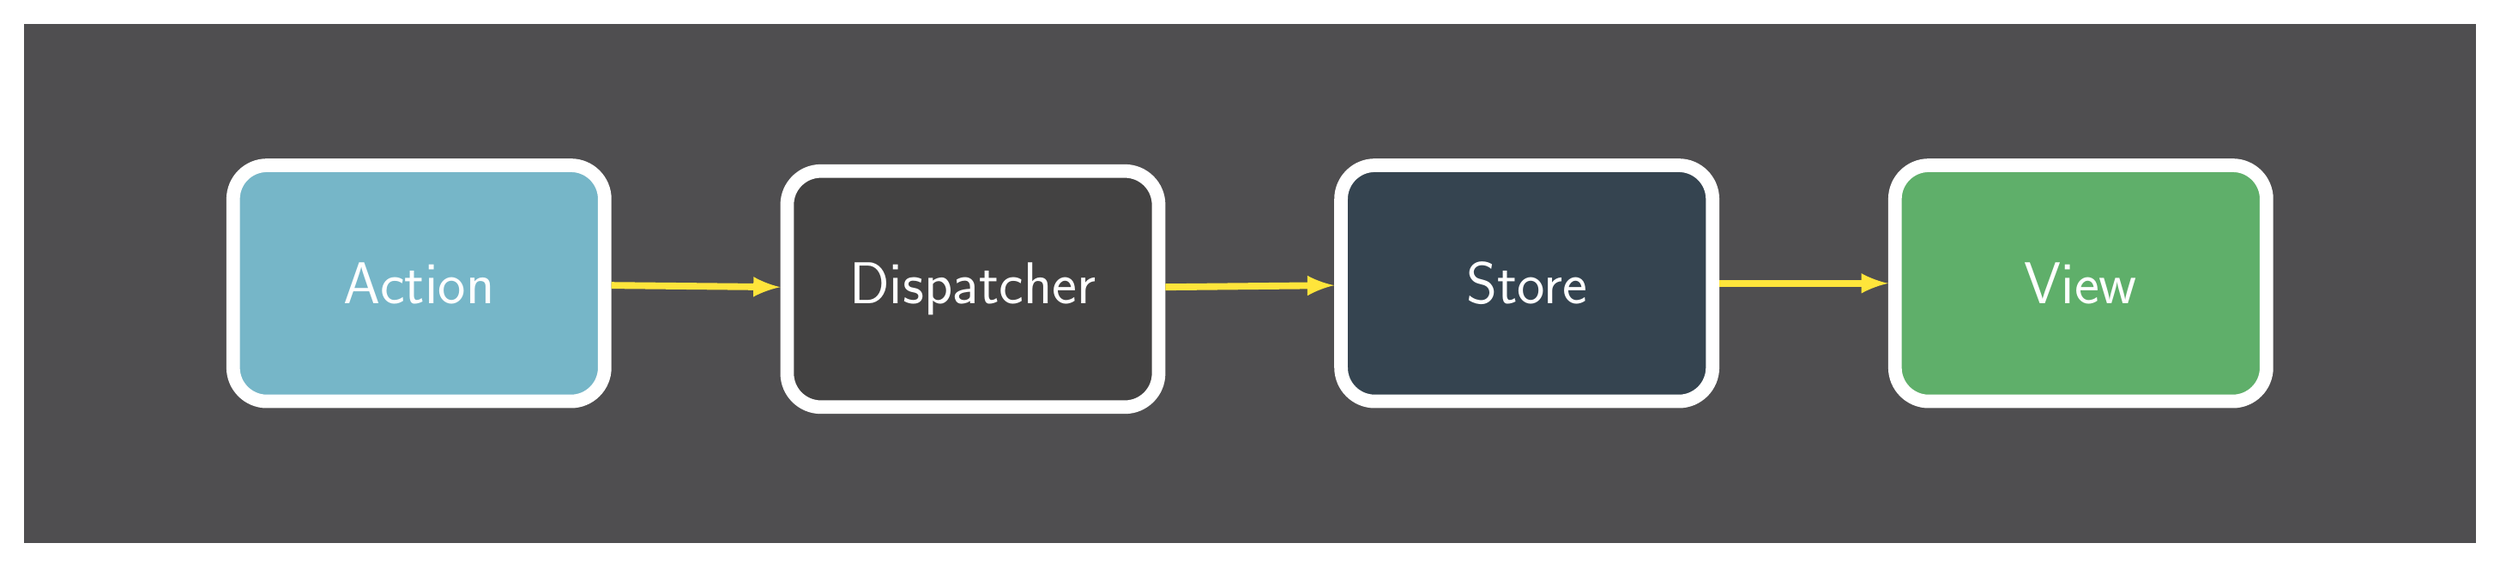
\begin{tikzpicture}
  \basediagram

  \begin{scope}[on background layer]
    \node [background,fit=(action) (view)] {};
  \end{scope}
\end{tikzpicture}
\endpgfgraphicnamed

\beginpgfgraphicnamed{flux-simple-f8-diagram-with-client-action}%
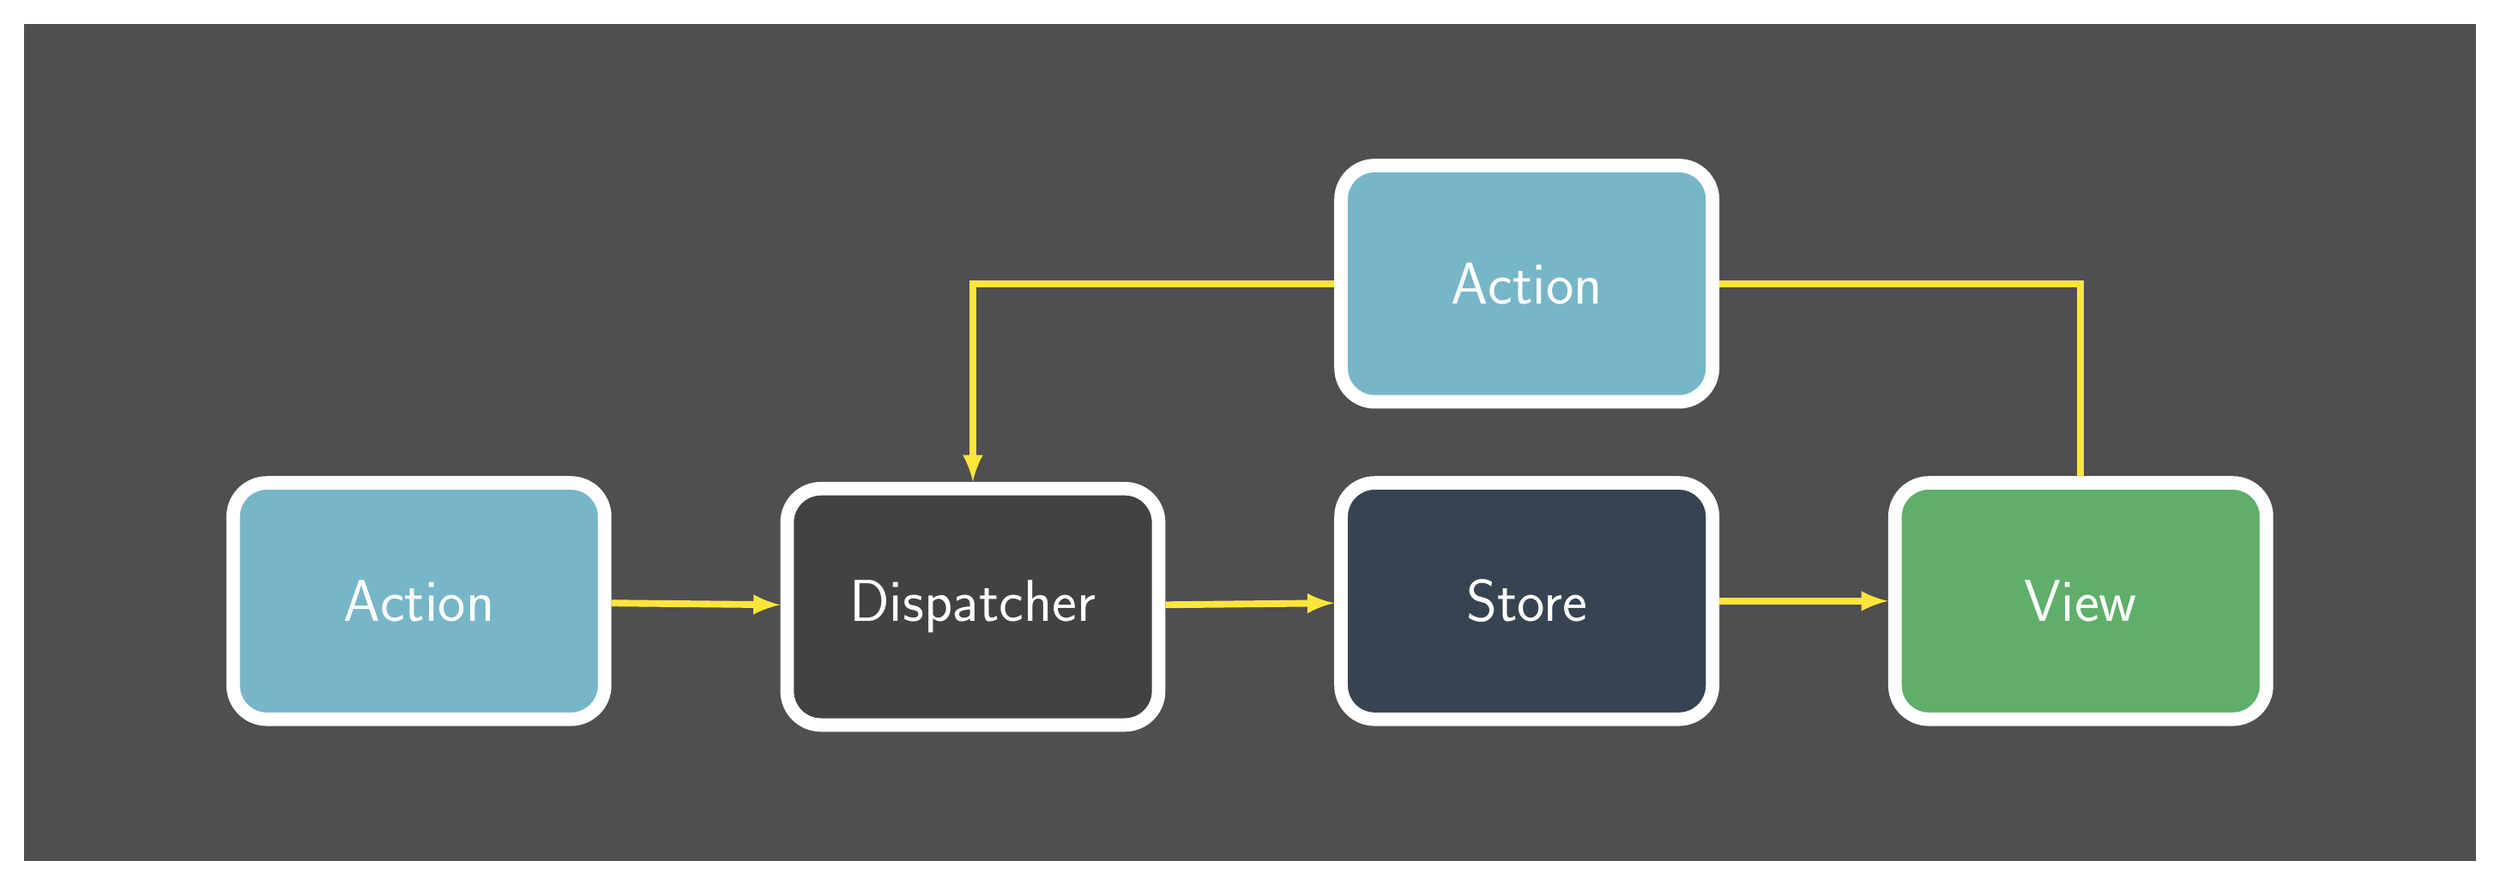
\begin{tikzpicture}
  \diagram

  \begin{scope}[on background layer]
    \node [background,fit=(action) (view) (action2)] {};
  \end{scope}
\end{tikzpicture}
\endpgfgraphicnamed

\beginpgfgraphicnamed{flux-simple-f8-diagram-explained}%
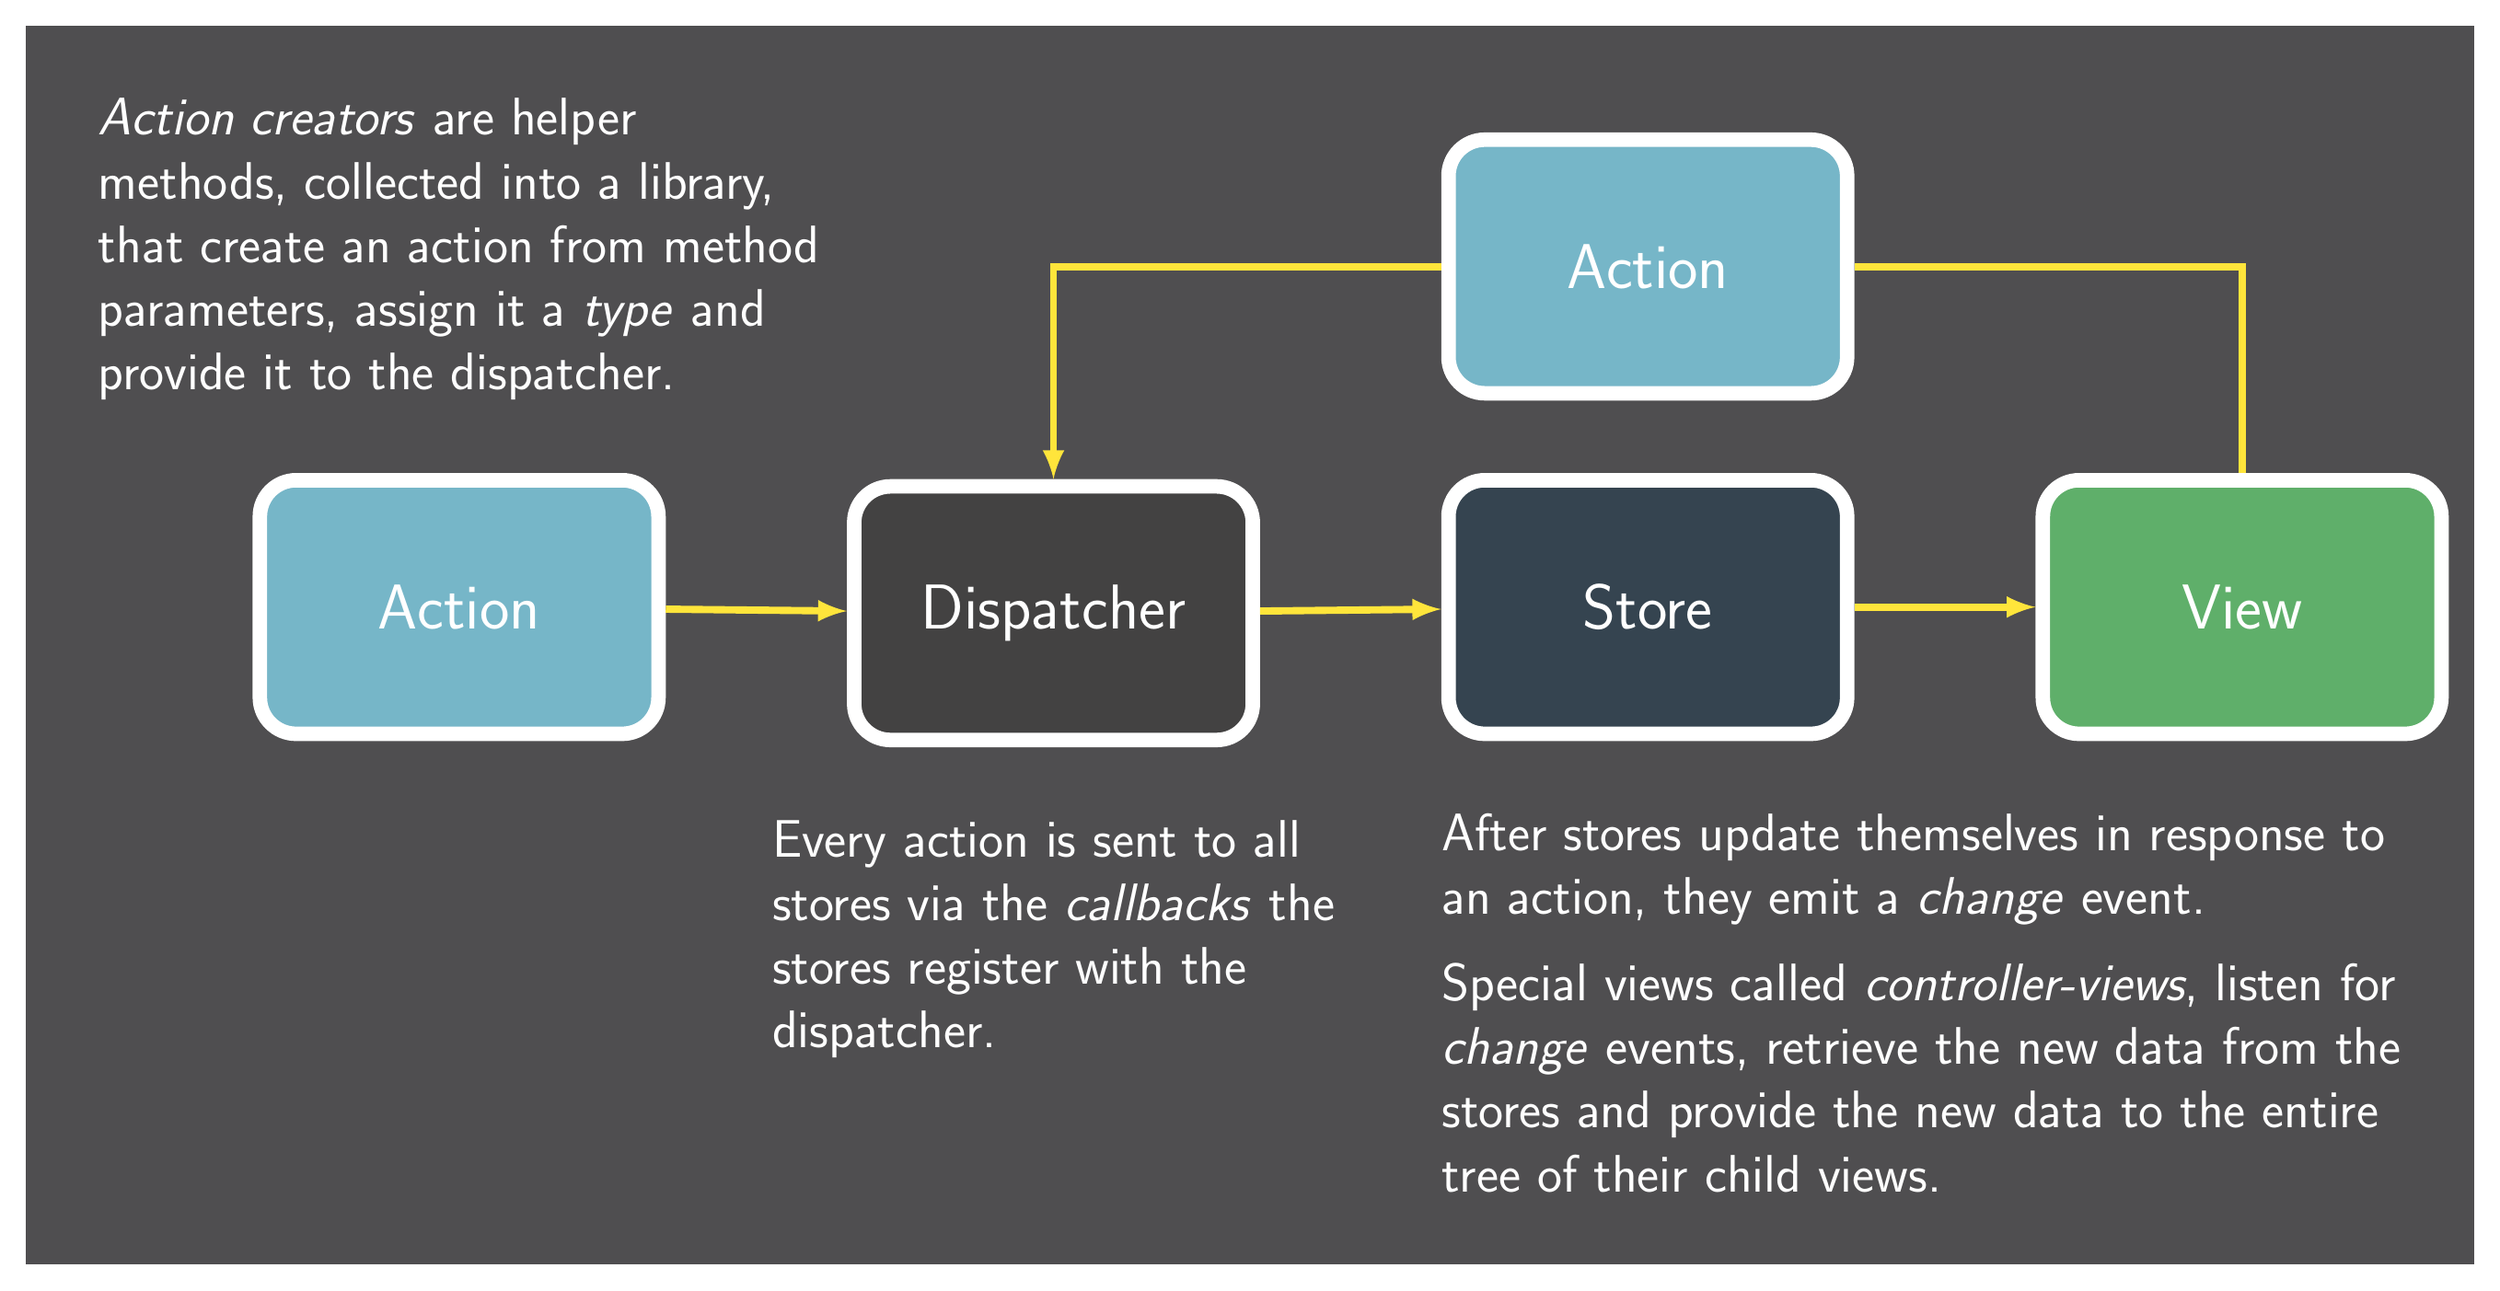
\begin{tikzpicture}
  \diagram

  \node (action explained) [explained,above=10mm of action] {%
    \textsl{Action creators} are helper\\
    methods, collected into a library,\\
    that create an action from method\\
    parameters, assign it a \textsl{type} and\\
    provide it to the dispatcher.};

  \node (dispatcher explained) [explained,below=10mm of dispatcher] {%
    Every action is sent to all\\
    stores via the \textsl{callbacks} the\\
    stores register with the\\
    dispatcher.};

  \node (store view explained) [explained,below=10mm,anchor=north west] at (store.south west) {%
    After stores update themselves in response to\\
    an action, they emit a \textsl{change} event.\\[1ex]
    Special views called \textsl{controller-views}, listen for\\
    \textsl{change} events, retrieve the new data from the\\
    stores and provide the new data to the entire\\
    tree of their child views.};

  \begin{scope}[on background layer]
    \node [background,inner sep=10mm,fit=(action explained) (store view explained)] {};
  \end{scope}
\end{tikzpicture}
\endpgfgraphicnamed

\beginpgfgraphicnamed{flux-simple-f8-diagram-explained-ja}%
\begin{tikzpicture}
  \node (action)     [action]                          {アクション};
  \node (dispatcher) [dispatcher,base right=of action] {ディスパッチャ};
  \node (store)      [store,base right=of dispatcher]  {ストア};
  \node (view)       [view,base right=of store]        {ビュー};
  \node (action2)    [action, above=10mm of store]     {アクション};

  \path [flow] (action) -- (dispatcher);
  \path [flow] (dispatcher) -- (store);
  \path [flow] (store) -- (view);
  \path [flow] (view) |- (action2) -| (dispatcher);

  \node (action explained) [explained,above=10mm of action,text width=140mm] {%
    \textsl{アクションクリエイタ}はヘルパーメソッドであり、ライブラリとして
    まとめられ、メソッドパラメータからアクションを作成し、\textsl{型}を割り当て、ディスパッチャに提供する。};

  \node (dispatcher explained) [explained,below=10mm of dispatcher,text width=85mm] {%
    各アクションは、ストアがディスパッチャに登録する\textsl{コールバック}を通して、すべてのストアに送られる。};

  \node (store view explained) [explained,below=10mm,anchor=north west,text width=150mm] at (store.south west) {%
    アクションの反応としてストアが自身を更新した後で、\textsl{change} イベントを発生させる。\\[1ex]
    \textsl{コントローラビュー}と呼ばれる特別なビューが \textsl{change} イベントをリッスンし、ストアから新しいデータを受信し、その新しいデータを子のビューツリー全体に提供する。};

  \begin{scope}[on background layer]
    \node [background,inner sep=10mm,fit=(action explained) (store view explained)] {};
  \end{scope}
\end{tikzpicture}
\endpgfgraphicnamed

\end{document}
